\documentclass[a4paper,11pt]{article}
\usepackage{fullpage}
\usepackage[latin1]{inputenc}
\usepackage[T1]{fontenc}
\usepackage[normalem]{ulem}
\usepackage[english]{babel}
\usepackage{listings,babel}
\lstset{breaklines=true,basicstyle=\ttfamily}
\usepackage{graphicx}
\usepackage{moreverb}
\usepackage{float}
\usepackage{url}
\usepackage{tabularx}

\title{Milkymist\texttrademark~ One testing procedure}
\author{S\'ebastien Bourdeauducq}
\date{November 2010}
\begin{document}
\setlength{\parindent}{0pt}
\setlength{\parskip}{5pt}
\maketitle{}


\section{Preparing the board}
\subsection{Flashing}
Prior to running the test program, the board should be flashed. At least the Milkymist SoC bitstream and the BIOS must be present, but, as part of the normal production process, other data is typically present in the flash memory as well.

Flashing instructions are available at \url{http://www.milkymist.org/wiki/index.php?title=Flashing_the_Milkymist_One}.

\subsection{Set-up}
For successfully running all the tests, the following hardware set-up is needed:
\begin{enumerate}
\item A 3.3V serial cable must be connected to the serial header of the board. This cable is used to transfer the automated testing program to the board and to control it.
\item The board must be connected to a VGA monitor with DDC (EDID) support.
\item A memory card must be installed in the reader of the board. The memory card must contain a conventional bootsector (i.e. that ends with \verb!0x55AA!).
\item An audio source must be available to feed the line input of the board.
\item An audio amplifier must be connected to the line output of the board.
\item The board must be on an Ethernet network with a computer responding to the IP address \verb!192.168.0.14!.
\item A video source must be connected to the board's video input connector.
\item The MIDI ports must be connected together (loopback) with a standard MIDI cable, preferably of the maximum length specified by the standard (15m).
\item The DMX ports must be connected together (loopback).
\item A RC5 remote control must be available to trigger the infrared sensor.
\item An USB keyboard must be available to test the host controller.
\end{enumerate}

\section{Compiling the automated testing program}
This section can be skipped if a pre-compiled testing program is available.
\subsection{Installing clang}
Clang (LLVM) is needed to compile some tools used in the Milkymist SDK. It is a standard package available in most Linux distributions.
\subsection{Installing the LM32 toolchain}
LM32 toolchain binaries can be downloaded from \url{http://www.milkymist.org/mmsoc.html}. Debian packages are also available, and can be installed by adding the following line to /etc/apt/sources.list:
\begin{verbatim}
deb http://www.milkymist.org/debian/ ./
\end{verbatim}
Then, the LM32 toolchain can be installed with \verb!apt-get install gcc-lm32!.

It is also possible to compile a GCC 4.5+ toolchain by following the usual procedure and configuring the toolchain as \verb!lm32-elf! without built-in C library.

\subsection{Building the Milkymist SDK}
First, you need to obtain a copy of the Milkymist SoC source distribution and unpack it. It can be downloaded from \url{http://www.milkymist.org/mmsoc.html}.

Then, cd to the uncompressed folder and enter:
\begin{verbatim}
export MMDIR=`pwd`
./build_sdk.sh
\end{verbatim}

\subsection{Building the testing program}
With the \verb!MMDIR! environment variable still set, go to the src folder of the source distribution of the testing program and enter \verb!make!. This will build the file boot.bin to be loaded into the board.

\section{Loading the automated testing program}
The tool \verb!flterm! is used. If you have built the Milkymist SDK, a copy is available as \$MMDIR/tools/flterm. It can also be installed in Debian (with the Milkymist repository configured) with:
\begin{verbatim}
apt-get install flterm
\end{verbatim}

Once \verb!flterm! is installed, loading the testing program is done with: (assuming \verb!/dev/ttyUSB0! is the device name of your serial cable)
\begin{verbatim}
flterm --port /dev/ttyUSB0 --kernel boot.bin
\end{verbatim}

The board will automatically download and run the program from \verb!flterm! during its boot sequence after a power-up or reset.

\section{Description of the tests}
\subsection{SDRAM}
\subsubsection{Address (A*) tests}
Those tests verify the connectivity of the SDRAM address lines by writing a word at one address, toggling the tested address line, and then writing a different word. The two words are then read back and verified.

The tests operate on the column address lines A8 to A12. The bank address lines and A0-A7 have already been tested by the 4MB test performed by the BIOS.

\subsubsection{Random pattern}
This test fills a memory buffer with pseudo-random data, reads it back and check that the data was not changed.

\subsubsection{Hammer pattern}
The principle is the same as the previous test, but the written pattern is alternatively \verb!0x00000000! and \verb!0xffffffff!. This is meant to electrically stress the SDRAM interface by inducing a large number of simultaneously switching outputs (SSOs).

\subsubsection{Crosstalk pattern}
The pattern used is alternatively \verb!0xaaaaaaaa! and \verb!0x55555555!. This electrically stresses the SDRAM interface to test the absence of crosstalk issues.

\subsection{GPIO}
\subsubsection{Switch tests}
The switch tests wait for each pushbutton to be pressed and released. If a pushbutton does not respond, the command \verb!f! can be typed to mark the test as failed. If the pushbutton test is not desired, it can be skipped with the command \verb!s!.

\subsubsection{LED tests}
The LED tests light each LED in turn and asks if it was correctly lit. The tests can be skipped by typing \verb!s!.

\subsection{VGA}
\subsubsection{DDC}
The test attempts to read the EDID of the connected monitor and checks if its header is correct. The correct EDID header is:
\begin{verbatim}
00 FF FF FF FF FF FF 00
\end{verbatim}

\subsubsection{Test card}
The test displays a test card on the monitor (figure~\ref{testcard}) and asks if it is correctly rendered.

\begin{figure}
\centering
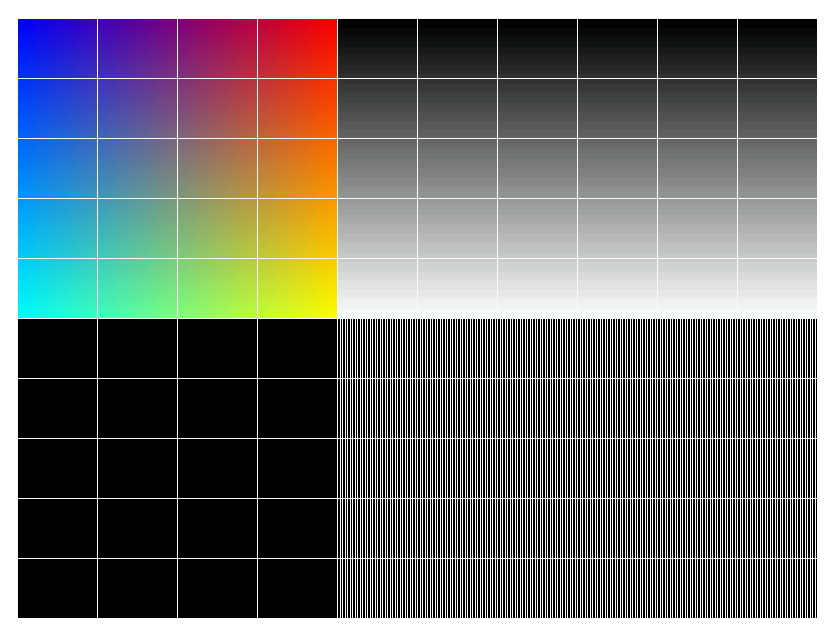
\includegraphics[width=\textwidth]{testcard.eps}
\caption{VGA test card.} \label{testcard}
\end{figure}

\subsection{Memory card}
\subsubsection{Card initialization}
The test performs the initialization of the memory card and checks that the card answers correctly. It basically checks the clocking and command lines of the memory card.

\subsubsection{Block read}
The test reads the first block of the card (block 0) and checks that it ends with \verb!0x55AA! (as a regular bootsector does). It exercises all the signals between the memory card and the FPGA.

\subsection{Audio}
\subsubsection{Codec probe}
The test checks for the presence of the LM4550 identification number in the AC97 identification register.

\subsubsection{Line and headphones output}
The test plays a 400Hz sine wave tone for one second and asks if it was correctly rendered. The command \verb!s! can be used to skip the test and the command \verb!r! to play the tone again.

\subsubsection{Microphone}
Approximately one second of audio is recorded from the built-in microphone, then played back. The test then asks if the sound was heard back. The command \verb!s! can be used to skip the test and the command \verb!r! to start over.

\subsubsection{Line input}
This is the same test as above, but with the line input.

\subsection{Ethernet}
\subsubsection{MDIO}
This checks if the KSZ8001 identification number can be read over the MDIO link.

\subsubsection{ARP resolution}
This test exercises packet transmission and reception by attempting an ARP resolution of the IP address \verb!192.168.0.14!. The board has the IP address \verb!192.168.0.42! for this test.

Any computer normally configured with the IP address \verb!192.168.0.14! should answer the ARP request coming from the board.

\subsection{Video input}
\subsubsection{Decoder probe}
This reads the identification register of the ADV7181 video chip and verifies its value.

\subsubsection{Capture}
This test attempts to capture one video frame, display it and asks if it is correctly rendered. Because of interlacing, the height of the captured picture is divided by two, and the resulting aspect ratio is not corrected by the test.

While waiting for the frame to be captured, the \verb!s! and \verb!f! keys can be used to skip and fail the test, respectively.

\subsection{MIDI}
The test sends the 256 possible values of the bytes used in the MIDI protocol, and check that they are correctly received back. The MIDI input and output connectors of the board must be connected together for this test.

\subsection{DMX512}
The test sets the 512 DMX channels of the transmitter to a pre-defined pattern, and check that the channel values are correctly received back by the receiver. The DMX input and output connectors of the board must be connected together for this test.

\subsection{Infrared}
The test waits for a "power off" RC5 code to be received. The device identification bits of the RC5 codes are ignored, so most RC5 remote controls can be used to perform the test. If the IR sensor does not respond, the command \verb!f! can be typed to mark the test as failed. If the IR test is not desired, it can be skipped with the command \verb!s!.

\subsection{USB}
The test waits for the \verb!ENTER! key to be pressed on a USB keyboard connected to each port, in turn.

While waiting for the \verb!ENTER! key to be pressed, the \verb!s! and \verb!f! keys can be used to skip and fail the test, respectively.

\section{Example session}
\begin{verbatim}
libHPDMC SDRAM initialization runtime
(c) Copyright 2010 Sebastien Bourdeauducq, released under GNU LGPL version 3.
Version 0.8

Initialization sequence completed.
Autocalibration OK, testing memory...
All SDRAM initialization completed, boot continuing.


MILKYMIST(tm) v0.8 BIOS http://www.milkymist.org
(c) Copyright 2007, 2008, 2009, 2010 Sebastien Bourdeauducq

This program is free software: you can redistribute it and/or modify
it under the terms of the GNU General Public License as published by
the Free Software Foundation, version 3 of the License.

I: BIOS CRC passed (d851470b)
I: Running on Milkymist One
I: Mem. card : Yes
I: AC'97     : Yes
I: PFPU      : Yes
I: TMU       : Yes
I: Ethernet  : Yes
I: FML meter : Yes
I: Video in  : Yes
I: MIDI      : Yes
I: DMX       : No
I: IR        : Yes
I: USB       : Yes
I: Displaying splash screen...OK
I: Press Q to abort boot
I: Attempting serial firmware loading
sL5DdSMmkekro
[FLTERM] Received firmware download request from the device.
[FLTERM] Uploading kernel (46808 bytes)...
[FLTERM] Upload complete (9.3KB/s).
[FLTERM] Booting the device.
[FLTERM] Done.
*** Milkymist One automated tests starting...

*** Running tests in category: SDRAM
Random pattern:                                            [  PASSED  ]
Hammer pattern:                                            [  PASSED  ]
Crosstalk pattern:                                         [  PASSED  ]

*** Running tests in category: GPIO
SW1:
Press the button. f to fail test, s to skip.               [  PASSED  ]
SW2:
Press the button. f to fail test, s to skip.               [  PASSED  ]
SW3:
Press the button. f to fail test, s to skip.               [  PASSED  ]
LED2:
Is the LED on? (y/n/s)                                     [  PASSED  ]
LED3:
Is the LED on? (y/n/s)                                     [  PASSED  ]

*** Running tests in category: VGA
DDC:
No ack for 0xA0 address                                    [  FAILED  ]
Test card:
Is the picture OK? (y/n/s)                                 [  PASSED  ]

*** Running tests in category: Memory card
Card initialization:                                       [  PASSED  ]
Block read:                                                [  PASSED  ]

*** Running tests in category: Audio
Codec probe:                                               [  PASSED  ]
Line and headphones outputs:
Is the test tone OK? (y/n/s/r)                             [  PASSED  ]
Microphone:
Recording...Playing...
Is the audio played back? (y/n/s/r)                        [  PASSED  ]
Line input:
Recording...Playing...
Is the audio played back? (y/n/s/r)                        [  PASSED  ]

*** Running tests in category: Ethernet
MDIO:                                                      [  PASSED  ]
ARP resolution:                                            [  FAILED  ]

*** Running tests in category: Video input
Decoder probe:                                             [  SKIPPED  ]
Capture:                                                   [  SKIPPED  ]

*** Running tests in category: MIDI
Loopback:                                                  [  PASSED  ]

*** Running tests in category: DMX512
Loopback:                                                  [  SKIPPED  ]

*** Running tests in category: Infrared
RC5 reception:
Waiting for remote. f to fail test, s to skip.             [  PASSED  ]

*** Running tests in category: USB
Full speed device enumeration (port A):                    [  SKIPPED  ]
Full speed device enumeration (port B):                    [  SKIPPED  ]
Low speed device enumeration (port A):                     [  SKIPPED  ]
Low speed device enumeration (port B):                     [  SKIPPED  ]

******** TEST SUMMARY ********
Failed tests:
  - VGA/DDC
  - Ethernet/ARP resolution

Skipped tests: 7
Failed tests:  2
Passed tests:  18
Total tests:   27

******** SOME TESTS FAILED ********
******** THERE WERE SOME SKIPPED TESTS ********
*** Power off/reset board now...
\end{verbatim}

\section*{Copyright notice}
Copyright \copyright 2010 S\'ebastien Bourdeauducq. \\
Permission is granted to copy, distribute and/or modify this document under the terms of the GNU Free Documentation License, Version 1.3; with no Invariant Sections, no Front-Cover Texts, and no Back-Cover Texts. A copy of the license is included in the LICENSE.FDL file at the root of the source distribution.

The testing program is free software: you can redistribute it and/or modify it under the terms of the GNU General Public License as published by the Free Software Foundation, version 3 of the License. A copy of the license is included in the LICENSE.GPL file at the root of the source distribution.

Milkymist is a trademark of S\'ebastien Bourdeauducq, which is not licensed under the GNU Free Documentation License nor the GNU General Public License.

\end{document}
